% uklad dokumentu
	\documentclass{article}
	\usepackage{xparse}
	\usepackage[margin=1cm]{geometry}
    \usepackage{enumerate} 
	\frenchspacing
    \linespread{1.2}
    \setlength{\parindent}{0pt}

% jezyk polski
	\usepackage[polish]{babel}
	\usepackage[utf8]{inputenc}
	\usepackage{polski}
 
% pakiety matematyczne
    \let\lll\undefined
	\usepackage{amssymb}
    \usepackage{amsthm}
	\usepackage{amsmath}
	\usepackage{amsfonts}
	\usepackage{tikz}

% hiperlacza
	\usepackage{hyperref}
	\hypersetup{
		colorlinks,
		citecolor=black,
		filecolor=black,
		linkcolor=black,
		urlcolor=black
	}

% wstawianie zdjec
	\usepackage{graphicx} 
	\pagenumbering{gobble}
	

% podstawowe informacje
    \title{Algorytmy metaheurystyczne 2}
    \author{Paweł Cegieła, Wojciech Sęk}

\begin{document} 

\maketitle

\section{Teoretyczna złożoność}
Warunkiem wyjścia w naszym algorytmie było przekroczenie $15n$ iteracji, gdzie $n=|V|$ lub $n$ ruchów bez zmiany na lepsze rozwiązanie. Rozważmy najgorszy możliwy przypadek, gdzie wykonujemy $15n$ iteracji. Niech $k$ to długość listy tabu. Implementacja listy tabu za pomocą VecDeq pozwala na dostęp do $i$-tego elementu w czasie stałym, a usuwanie i dodawanie elementów w czasie liniowym.
\\
W każdym kroku algorytmu przeglądamy wszystkich $\frac{n(n-1)}{2}$ sąsiadów danego rozwiązania i dla każdego sprawdzamy z $O(k)$ czy jest na liście tabu. Sprawdzenie o ile sąsiad zmienia wartość permutacji jest stały (dla $invert$ liczymy wcześniej z $O(n^2)$ pomocnicze tablice. Niech $O(l)$ to złożoność przybliżenia początkowego (dla 
2-$opt$ $O(n^3)$. Wybieramy najlepszego z nich. Ostatecznie mamy (dla $k$ stałego i  $2$-opta):
$$O\left(15n\cdot \frac{n(n-1)}{2} \cdot k + l\right)=O(n^3)$$


\section{Porównanie Tabu Search z 2-OPT}

\subsection{Dane z TSPLIB}

\subsubsection{Grafy asymetryczne}
\begin{center}
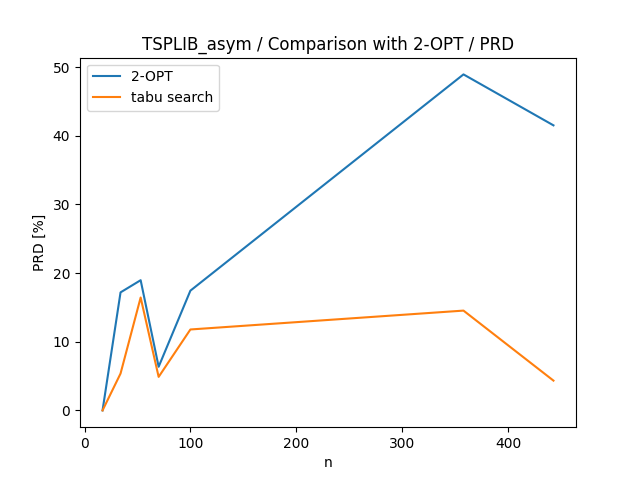
\includegraphics[width=\textwidth, 
                   height = 0.4\textheight, 
                   keepaspectratio]
                  {plots/two_opt_tsplib_asym_prd} 
\end{center}


\subsubsection{Grafy euklidesowe}

\begin{center}
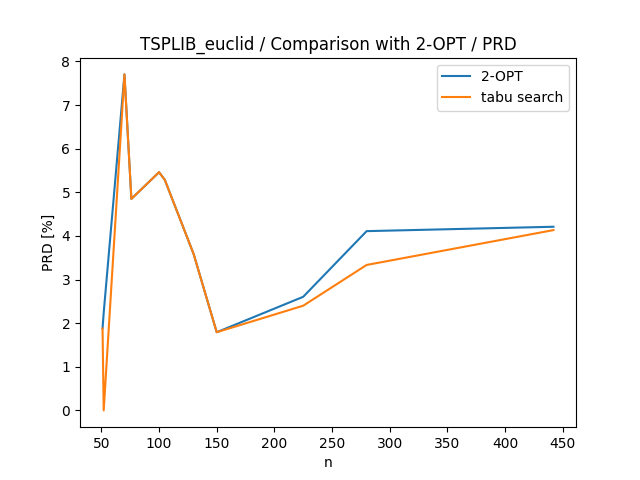
\includegraphics[width=\textwidth, 
                   height = 0.4\textheight, 
                   keepaspectratio]
                  {plots/two_opt_tsplib_euclid_prd} 
\end{center}


\subsection{Dane generowane przez nas}


\subsubsection{Grafy symetryczne}

\begin{center}
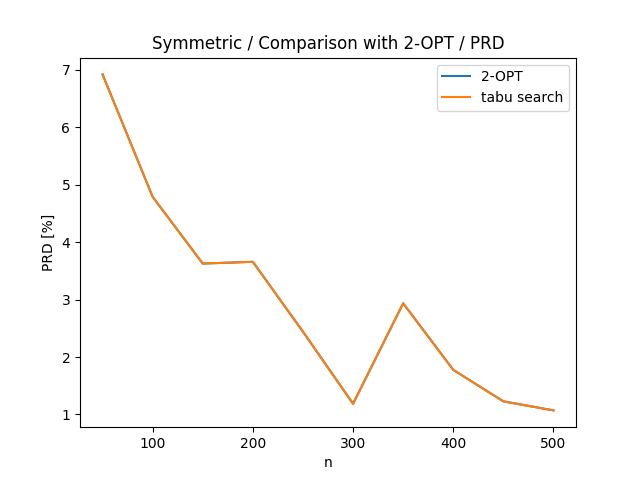
\includegraphics[width=\textwidth, 
                   height = 0.4\textheight, 
                   keepaspectratio]
                  {plots/two_opt_symmetric_prd} 
\end{center}

\subsubsection{Grafy asymetryczne}

\begin{center}
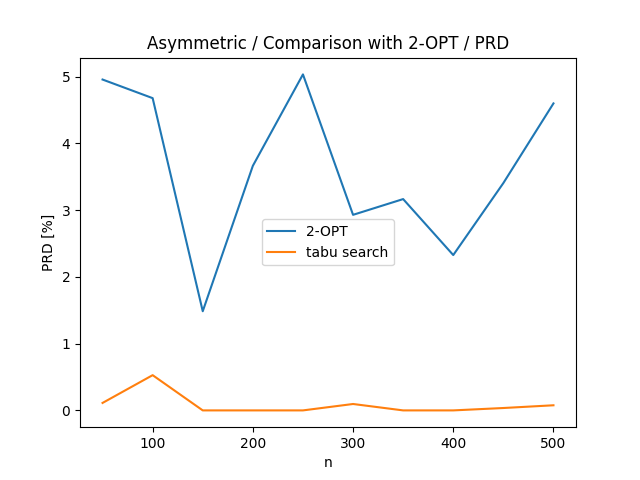
\includegraphics[width=\textwidth, 
                   height = 0.4\textheight, 
                   keepaspectratio]
                  {plots/two_opt_asymmetric_prd} 
\end{center}


\subsubsection{Grafy euklidesowe}

\begin{center}
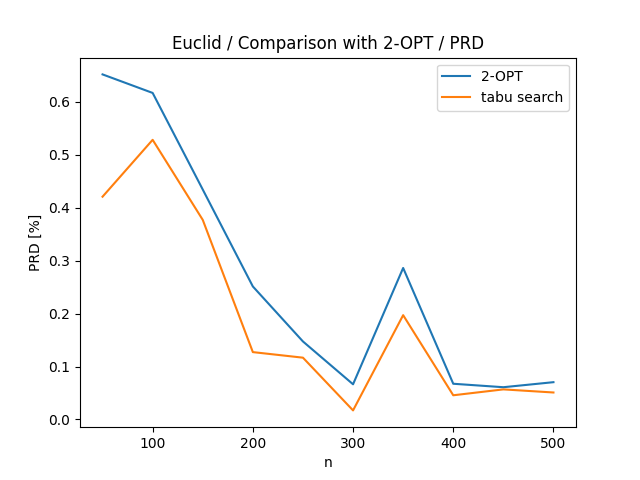
\includegraphics[width=\textwidth, 
                   height = 0.4\textheight, 
                   keepaspectratio]
                  {plots/two_opt_euclid_prd} 
\end{center}


\subsection{Obserwacje}

Dla każdego typu grafów Tabu Search zwraca przynajmniej tak samo dobre, a najczęściej lepsze wyniki od 2-OPT, na którym bazuje.

W przypadku grafów asymetrycznych, różnica w PRD pomiędzy Tabu Search a 2-OPT jest największa. Grafy euklidesowe są w dalszym ciągu przeszukiwane lepiej przez Tabu Search, ale różnica jest już minimalna. Dla grafów symetrycznych wyniki pokrywały się.


\subsection{Tabele}

\begin{center}
\begin{tabular}{|c|c|c|}
\hline
\multicolumn{3}{|c|}{\textbf{Asymmetric / Comparison with 2-OPT / PRD}}\\
\hline
\textbf{n} & 2-OPT & Tabu Search\\
\hline
50 & 0.11191047162270185 & 0.11191047162270185\\
\hline
100 & 0.52807735217553 & 0.52807735217553\\
\hline
150 & 0.0 & 0.0\\
\hline
200 & 0.0 & 0.0\\
\hline
250 & 0.0 & 0.0\\
\hline
300 & 0.09599191647019198 & 0.09599191647019198\\
\hline
350 & 0.0 & 0.0\\
\hline
400 & 0.0 & 0.0\\
\hline
450 & 0.03581064508216826 & 0.03581064508216826\\
\hline
500 & 0.0766979513573519 & 0.0766979513573519\\
\hline
\end{tabular}
\end{center}


\begin{center}
\begin{tabular}{|c|c|c|}
\hline
\multicolumn{3}{|c|}{\textbf{Euclid / Comparison with 2-OPT / PRD}}\\
\hline
\textbf{n} & 2-OPT & Tabu Search\\
\hline
50 & 0.4207549708890032 & 0.4207549708890032\\
\hline
100 & 0.5282007435256711 & 0.5282007435256711\\
\hline
150 & 0.3769823007501678 & 0.3769823007501678\\
\hline
200 & 0.1271843910979231 & 0.1271843910979231\\
\hline
250 & 0.11667189906458164 & 0.11667189906458164\\
\hline
300 & 0.017076672487704073 & 0.017076672487704073\\
\hline
350 & 0.19697835915506468 & 0.19697835915506468\\
\hline
400 & 0.04564711832989831 & 0.04564711832989831\\
\hline
450 & 0.056766273647667766 & 0.056766273647667766\\
\hline
500 & 0.050901971434817714 & 0.050901971434817714\\
\hline
\end{tabular}
\end{center}


\begin{center}
\begin{tabular}{|c|c|c|}
\hline
\multicolumn{3}{|c|}{\textbf{Symmetric / Comparison with 2-OPT / PRD}}\\
\hline
\textbf{n} & 2-OPT & Tabu Search\\
\hline
50 & 6.917692987893891 & 6.917692987893891\\
\hline
100 & 4.787518110638111 & 4.787518110638111\\
\hline
150 & 3.6259066537639213 & 3.6259066537639213\\
\hline
200 & 3.65693454118884 & 3.65693454118884\\
\hline
250 & 2.4413015900221464 & 2.4413015900221464\\
\hline
300 & 1.1869594271627262 & 1.1869594271627262\\
\hline
350 & 2.9343241182614768 & 2.9343241182614768\\
\hline
400 & 1.7767045918185538 & 1.7767045918185538\\
\hline
450 & 1.2285915175711815 & 1.2285915175711815\\
\hline
500 & 1.0711060843000912 & 1.0711060843000912\\
\hline
\end{tabular}
\end{center}


\begin{center}
\begin{tabular}{|c|c|c|}
\hline
\multicolumn{3}{|c|}{\textbf{TSPLIB asym / Comparison with 2-OPT / PRD}}\\
\hline
\textbf{n} & 2-OPT & Tabu Search\\
\hline
17 & 0.0 & 0.0\\
\hline
34 & 5.365474339035769 & 5.365474339035769\\
\hline
53 & 16.437364228819696 & 16.437364228819696\\
\hline
70 & 4.881958989475862 & 4.881958989475862\\
\hline
100 & 11.783052718741374 & 11.783052718741374\\
\hline
358 & 14.531384350816854 & 14.531384350816854\\
\hline
443 & 4.338235294117647 & 4.338235294117647\\
\hline
\end{tabular}
\end{center}


\begin{center}
\begin{tabular}{|c|c|c|}
\hline
\multicolumn{3}{|c|}{\textbf{TSPLIB euclid / Comparison with 2-OPT / PRD}}\\
\hline
\textbf{n} & 2-OPT & Tabu Search\\
\hline
51 & 1.8779342723004695 & 1.8779342723004695\\
\hline
52 & 0.0 & 0.0\\
\hline
70 & 7.703703703703704 & 7.703703703703704\\
\hline
76 & 4.849342172172451 & 4.849342172172451\\
\hline
100 & 5.461441213653603 & 5.461441213653603\\
\hline
105 & 5.285485777870505 & 5.285485777870505\\
\hline
130 & 3.5842880523731586 & 3.5842880523731586\\
\hline
150 & 1.7922794117647058 & 1.7922794117647058\\
\hline
225 & 2.400408580183861 & 2.400408580183861\\
\hline
280 & 3.3346258239627766 & 3.3346258239627766\\
\hline
442 & 4.133679940131553 & 4.133679940131553\\
\hline
\end{tabular}
\end{center}




\section{Porównanie różnych długości listy tabu}

\subsection{Dane z TSPLIB}

\subsubsection{Grafy asymetryczne}

\begin{center}
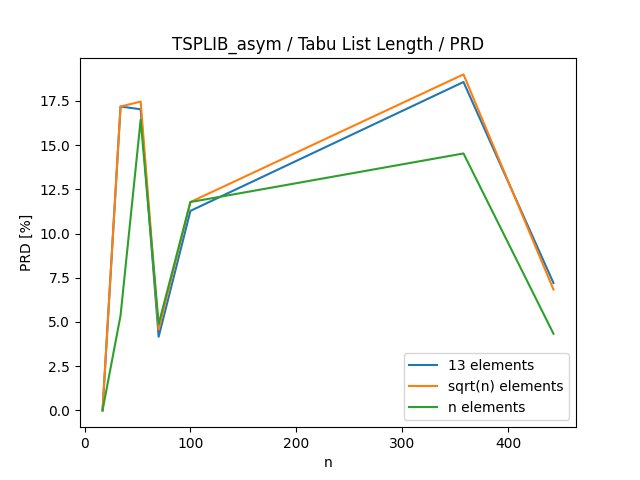
\includegraphics[width=\textwidth, 
                   height = 0.4\textheight, 
                   keepaspectratio]
                  {plots/tabu_tsplib_asym_prd} 
\end{center}

\begin{center}
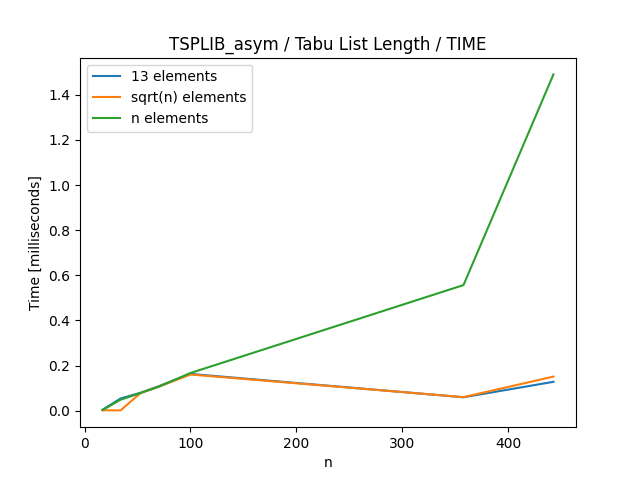
\includegraphics[width=\textwidth, 
                   height = 0.4\textheight, 
                   keepaspectratio]
                  {plots/tabu_tsplib_asym_time} 
\end{center}

\subsubsection{Grafy euklidesowe}

\begin{center}
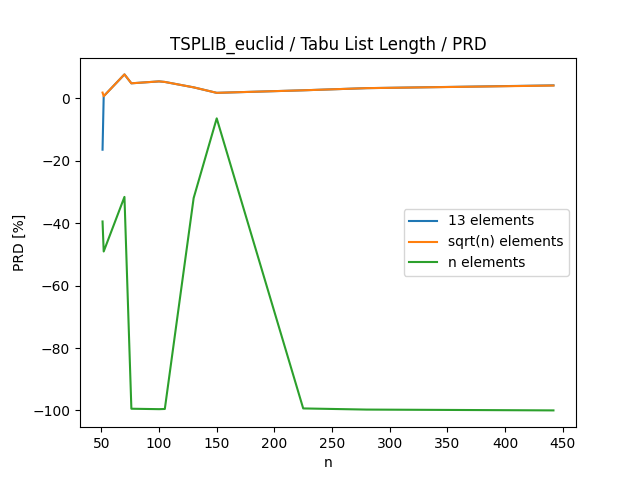
\includegraphics[width=\textwidth, 
                   height = 0.4\textheight, 
                   keepaspectratio]
                  {plots/tabu_tsplib_euclid_prd} 
\end{center}

\begin{center}
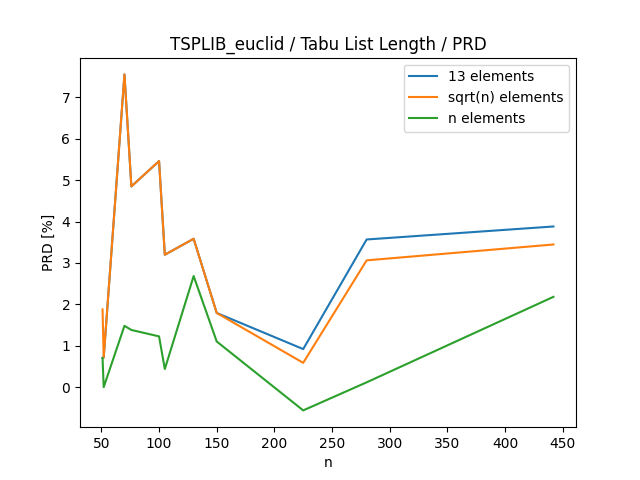
\includegraphics[width=\textwidth, 
                   height = 0.4\textheight, 
                   keepaspectratio]
                  {plots/tabu_tsplib_euclid_time} 
\end{center}


\subsection{Dane generowane przez nas}


\subsubsection{Grafy symetryczne}

\begin{center}
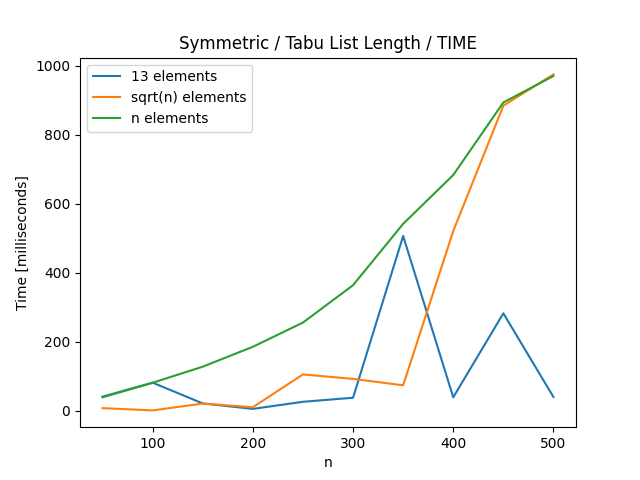
\includegraphics[width=\textwidth, 
                   height = 0.4\textheight, 
                   keepaspectratio]
                  {plots/tabu_symmetric_prd} 
\end{center}

\begin{center}
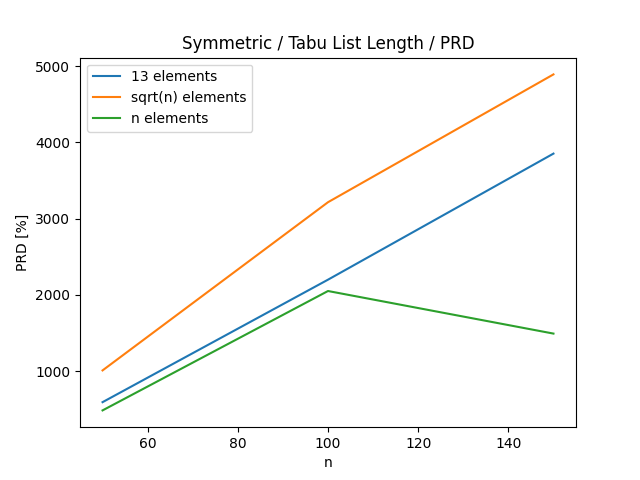
\includegraphics[width=\textwidth, 
                   height = 0.4\textheight, 
                   keepaspectratio]
                  {plots/tabu_symmetric_time} 
\end{center}

\subsubsection{Grafy asymetryczne}

\begin{center}
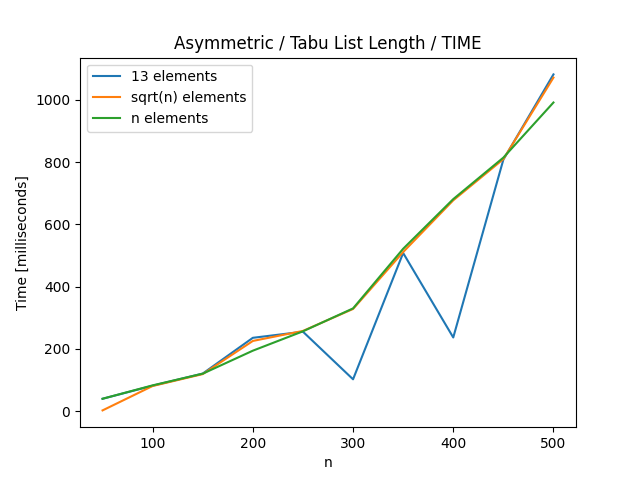
\includegraphics[width=\textwidth, 
                   height = 0.4\textheight, 
                   keepaspectratio]
                  {plots/tabu_asymmetric_prd} 
\end{center}

\begin{center}
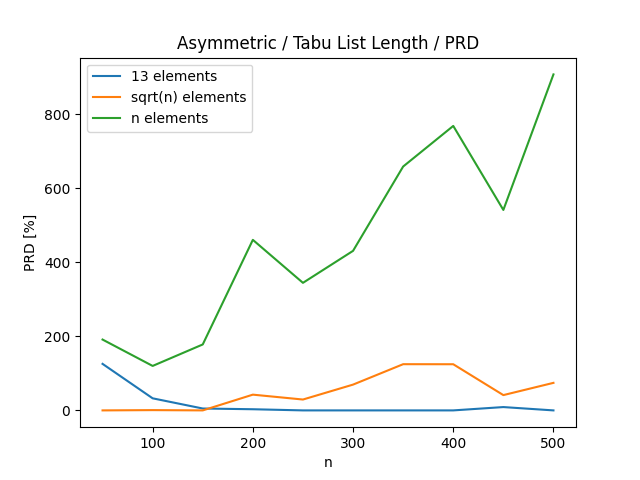
\includegraphics[width=\textwidth, 
                   height = 0.4\textheight, 
                   keepaspectratio]
                  {plots/tabu_asymmetric_time} 
\end{center}

\subsubsection{Grafy euklidesowe}

\begin{center}
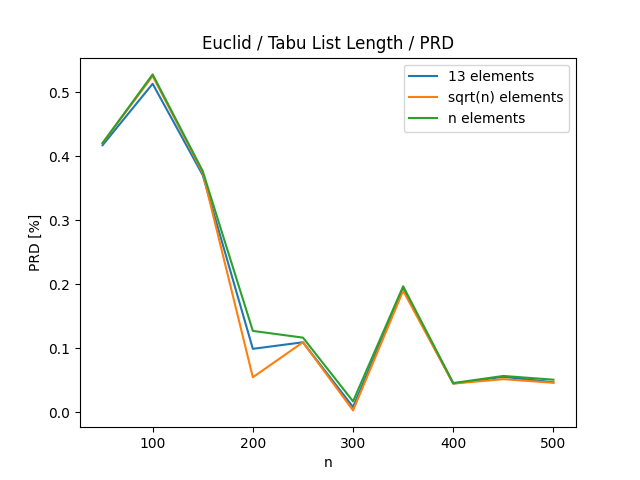
\includegraphics[width=\textwidth, 
                   height = 0.4\textheight, 
                   keepaspectratio]
                  {plots/tabu_euclid_prd} 
\end{center}

\begin{center}
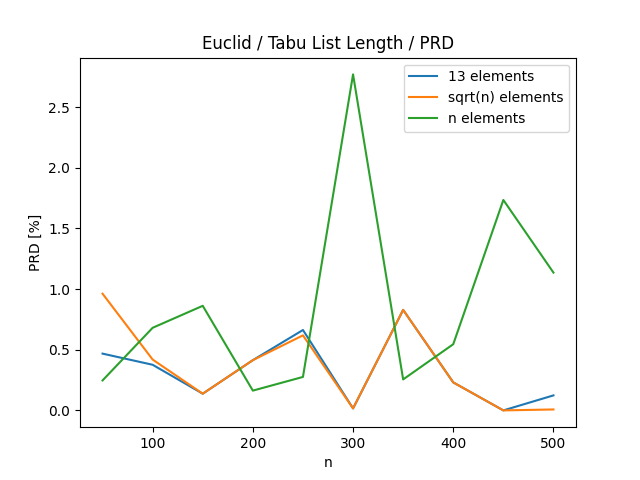
\includegraphics[width=\textwidth, 
                   height = 0.4\textheight, 
                   keepaspectratio]
                  {plots/tabu_euclid_time} 
\end{center}

\subsection{Obserwacje}

W przypadku grafów asymetrycznych z TSPLIB, najlepiej radził sobie algorytm z najdłuższą listą tabu - n-elementową (natomiast dla grafów generowanych, rezultaty dla wszystkich długości były takie same lub minimalnie lepsze dla 13 el.). Na grafach euklidesowych wyniki były zbliżone. Dla grafów symetrycznych nie było różnicy w wyborze długości listy tabu.

Jeśli chodzi o czas, dla każdego z przypadków najdłużej trwało przejście algorytmu dla najdłuższej listy tabu. W przypadku generowanych przez nas grafów symetrycznych i asymetrycznych, zbliżone czasy trwania miał algorytm z tabu o długości $\sqrt{n}$

\subsection{Tabele}

\begin{center}
\begin{tabular}{|c|c|c|c|}
\hline
\multicolumn{4}{|c|}{\textbf{Asymmetric / Tabu list length / PRD}}\\
\hline
\textbf{n} & 13 & $\sqrt{n}$ & n\\
\hline
50 & 0.11191047162270185 & 0.11191047162270185 & 0.11191047162270185\\
\hline
100 & 0.52807735217553 & 0.52807735217553 & 0.52807735217553\\
\hline
150 & 0.0 & 0.0 & 0.0\\
\hline
200 & 0.0 & 0.0 & 0.0\\
\hline
250 & 0.0 & 0.0 & 0.0\\
\hline
300 & 0.0 & 0.09599191647019198 & 0.09599191647019198\\
\hline
350 & 0.0 & 0.0 & 0.0\\
\hline
400 & 0.0 & 0.0 & 0.0\\
\hline
450 & 0.0 & 0.03581064508216826 & 0.03581064508216826\\
\hline
500 & 0.0 & 0.0766979513573519 & 0.0766979513573519\\
\hline
\end{tabular}
\end{center}


\begin{center}
\begin{tabular}{|c|c|c|c|}
\hline
\multicolumn{4}{|c|}{\textbf{Asymmetric / Tabu list length / Time}}\\
\hline
\textbf{n} & 13 & $\sqrt{n}$ & n\\
\hline
50 & 0.07385802999999999 & 0.028744079999999995 & 0.07376404\\
\hline
100 & 0.15944619999999998 & 0.10658849 & 0.16007074999999998\\
\hline
150 & 0.3033876 & 0.24521492999999994 & 0.31249241000000005\\
\hline
200 & 0.30667507999999993 & 0.48976515000000004 & 0.54841901\\
\hline
250 & 0.62445054 & 0.7853915999999999 & 0.8751694499999999\\
\hline
300 & 0.78834145 & 1.3305461199999997 & 1.34324706\\
\hline
350 & 0.8908741500000001 & 1.57709417 & 1.9484998399999998\\
\hline
400 & 1.31986308 & 2.72034879 & 2.74655025\\
\hline
450 & 1.38779908 & 3.7751664 & 3.801825290000001\\
\hline
500 & 1.5568623 & 4.5591865 & 5.08990898\\
\hline
\end{tabular}
\end{center}


\begin{center}
\begin{tabular}{|c|c|c|c|}
\hline
\multicolumn{4}{|c|}{\textbf{Euclid / Tabu list length / PRD}}\\
\hline
\textbf{n} & 13 & $\sqrt{n}$ & n\\
\hline
50 & 0.41747089863941367 & 0.4207549708890032 & 0.4207549708890032\\
\hline
100 & 0.513520849011387 & 0.5257261085343324 & 0.5282007435256711\\
\hline
150 & 0.3706918377833429 & 0.3742384401382869 & 0.3769823007501678\\
\hline
200 & 0.09916957017990424 & 0.05476201991278836 & 0.1271843910979231\\
\hline
250 & 0.10943361971724283 & 0.10943361971724283 & 0.11667189906458164\\
\hline
300 & 0.008143056907276255 & 0.002919636991800686 & 0.017076672487704073\\
\hline
350 & 0.19258345724128464 & 0.18991027309708547 & 0.19697835915506468\\
\hline
400 & 0.04483850563308839 & 0.04483850563308839 & 0.04564711832989831\\
\hline
450 & 0.055414537386798336 & 0.05175307680208402 & 0.056766273647667766\\
\hline
500 & 0.04684067228013384 & 0.04612221554882399 & 0.050901971434817714\\
\hline
\end{tabular}
\end{center}


\begin{center}
\begin{tabular}{|c|c|c|c|}
\hline
\multicolumn{4}{|c|}{\textbf{Euclid / Tabu list length / Time}}\\
\hline
\textbf{n} & 13 & $\sqrt{n}$ & n\\
\hline
50 & 0.06892951 & 0.02786071 & 0.07344694\\
\hline
100 & 0.10688875 & 0.07182816 & 0.16274169\\
\hline
150 & 0.16533177 & 0.13686594 & 0.3153742\\
\hline
200 & 0.39902903 & 0.4290532799999999 & 0.5656857900000001\\
\hline
250 & 0.5470563900000001 & 0.5496629700000001 & 0.89462399\\
\hline
300 & 0.3658269 & 0.7317911899999998 & 1.37161821\\
\hline
350 & 0.70801814 & 1.2293225500000002 & 2.0154079099999995\\
\hline
400 & 0.31940638 & 1.1810165700000002 & 2.8054042600000004\\
\hline
450 & 1.1279154999999998 & 1.94813256 & 3.8271469\\
\hline
500 & 1.79325678 & 2.76704791 & 5.11919333\\
\hline
\end{tabular}
\end{center}


\begin{center}
\begin{tabular}{|c|c|c|c|}
\hline
\multicolumn{4}{|c|}{\textbf{Symmetric / Tabu list length / PRD}}\\
\hline
\textbf{n} & 13 & $\sqrt{n}$ & n\\
\hline
50 & 6.917692987893891 & 6.917692987893891 & 6.917692987893891\\
\hline
100 & 4.787518110638111 & 4.787518110638111 & 4.787518110638111\\
\hline
150 & 3.6259066537639213 & 3.6259066537639213 & 3.6259066537639213\\
\hline
200 & 3.65693454118884 & 3.65693454118884 & 3.65693454118884\\
\hline
250 & 2.4413015900221464 & 2.4413015900221464 & 2.4413015900221464\\
\hline
300 & 1.1869594271627262 & 1.1869594271627262 & 1.1869594271627262\\
\hline
350 & 2.9343241182614768 & 2.9343241182614768 & 2.9343241182614768\\
\hline
400 & 1.7767045918185538 & 1.7767045918185538 & 1.7767045918185538\\
\hline
450 & 1.2285915175711815 & 1.2285915175711815 & 1.2285915175711815\\
\hline
500 & 1.0711060843000912 & 1.0711060843000912 & 1.0711060843000912\\
\hline
\end{tabular}
\end{center}


\begin{center}
\begin{tabular}{|c|c|c|c|}
\hline
\multicolumn{4}{|c|}{\textbf{Symmetric / Tabu list length / Time}}\\
\hline
\textbf{n} & 13 & $\sqrt{n}$ & n\\
\hline
50 & 0.07311498 & 0.03475836 & 0.07261012\\
\hline
100 & 0.15076814 & 0.14221727999999997 & 0.16149818\\
\hline
150 & 0.24539080000000002 & 0.23409864999999996 & 0.30667559000000005\\
\hline
200 & 0.27950255 & 0.4152889 & 0.54723579\\
\hline
250 & 0.4766900100000001 & 0.5219849499999999 & 0.8675596299999999\\
\hline
300 & 0.15507567 & 1.06678467 & 1.33364641\\
\hline
350 & 1.0168580200000001 & 1.4747576800000002 & 1.95661837\\
\hline
400 & 0.59430354 & 2.01161023 & 2.7663511699999996\\
\hline
450 & 1.2444358499999997 & 3.0308625499999997 & 3.79851777\\
\hline
500 & 1.8332309300000003 & 4.68484663 & 5.06103543\\
\hline
\end{tabular}
\end{center}


\begin{center}
\begin{tabular}{|c|c|c|c|}
\hline
\multicolumn{4}{|c|}{\textbf{TSPLIB asym / Tabu list length / PRD}}\\
\hline
\textbf{n} & 13 & $\sqrt{n}$ & n\\
\hline
17 & 0.0 & 0.0 & 0.0\\
\hline
34 & 17.1850699844479 & 17.1850699844479 & 5.365474339035769\\
\hline
53 & 17.031136857349747 & 17.465604634322954 & 16.437364228819696\\
\hline
70 & 4.165696997905515 & 4.57683655263362 & 4.881958989475862\\
\hline
100 & 11.283466740270494 & 11.783052718741374 & 11.783052718741374\\
\hline
358 & 18.572656921754085 & 19.002579535683576 & 14.531384350816854\\
\hline
443 & 7.205882352941176 & 6.838235294117648 & 4.338235294117647\\
\hline
\end{tabular}
\end{center}


\begin{center}
\begin{tabular}{|c|c|c|c|}
\hline
\multicolumn{4}{|c|}{\textbf{TSPLIB asym / Tabu list length / Time}}\\
\hline
\textbf{n} & 13 & $\sqrt{n}$ & n\\
\hline
17 & 0.0043833 & 0.0021721 & 0.0034579\\
\hline
34 & 0.0543166 & 0.0016518 & 0.0488397\\
\hline
53 & 0.0799956 & 0.0790441 & 0.0787211\\
\hline
70 & 0.10852 & 0.10629 & 0.1066343\\
\hline
100 & 0.1633046 & 0.1606365 & 0.1671848\\
\hline
358 & 0.0598049 & 0.060473 & 0.556717\\
\hline
443 & 0.128276 & 0.1514229 & 1.4899777\\
\hline
\end{tabular}
\end{center}


\begin{center}
\begin{tabular}{|c|c|c|c|}
\hline
\multicolumn{4}{|c|}{\textbf{TSPLIB euclid / Tabu list length / PRD}}\\
\hline
\textbf{n} & 13 & $\sqrt{n}$ & n\\
\hline
51 & 1.8779342723004695 & 1.8779342723004695 & 1.8779342723004695\\
\hline
52 & 0.0 & 0.7159904534606205 & 0.0\\
\hline
70 & 7.703703703703704 & 7.703703703703704 & 7.703703703703704\\
\hline
76 & 4.849342172172451 & 4.849342172172451 & 4.849342172172451\\
\hline
100 & 5.461441213653603 & 5.461441213653603 & 5.461441213653603\\
\hline
105 & 5.285485777870505 & 5.285485777870505 & 5.285485777870505\\
\hline
130 & 3.551554828150573 & 3.551554828150573 & 3.5842880523731586\\
\hline
150 & 1.7922794117647058 & 1.7922794117647058 & 1.7922794117647058\\
\hline
225 & 2.400408580183861 & 2.29826353421859 & 2.400408580183861\\
\hline
280 & 3.3346258239627766 & 3.450949980612641 & 3.3346258239627766\\
\hline
442 & 4.210484855646146 & 4.133679940131553 & 4.133679940131553\\
\hline
\end{tabular}
\end{center}


\begin{center}
\begin{tabular}{|c|c|c|c|}
\hline
\multicolumn{4}{|c|}{\textbf{TSPLIB euclid / Tabu list length / Time}}\\
\hline
\textbf{n} & 13 & $\sqrt{n}$ & n\\
\hline
51 & 0.0052827 & 0.0024253 & 0.0792794\\
\hline
52 & 0.0851107 & 0.002831 & 0.0793002\\
\hline
70 & 0.0332155 & 0.0026489 & 0.1098126\\
\hline
76 & 0.1232844 & 0.1115039 & 0.113911\\
\hline
100 & 0.0646367 & 0.1623564 & 0.1608226\\
\hline
105 & 0.1881329 & 0.1837667 & 0.1828318\\
\hline
130 & 0.2533528 & 0.11668 & 0.2498604\\
\hline
150 & 0.009127 & 0.0059214 & 0.3236019\\
\hline
225 & 0.6909736 & 0.0292159 & 0.6941704\\
\hline
280 & 0.0345763 & 0.0388206 & 1.1307793\\
\hline
442 & 0.0266773 & 0.1404226 & 3.5502116\\
\hline
\end{tabular}
\end{center}



\section{Porównanie sąsiedztwa insert i swap}

\subsection{Dane z TSPLIB}

\subsubsection{Grafy asymetryczne}

\begin{center}
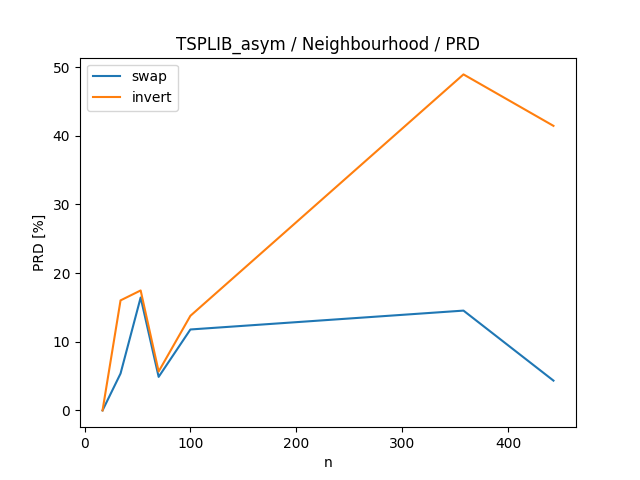
\includegraphics[width=\textwidth, 
                   height = 0.4\textheight, 
                   keepaspectratio]
                  {plots/neighbours_tsplib_asym_prd} 
\end{center}

\begin{center}
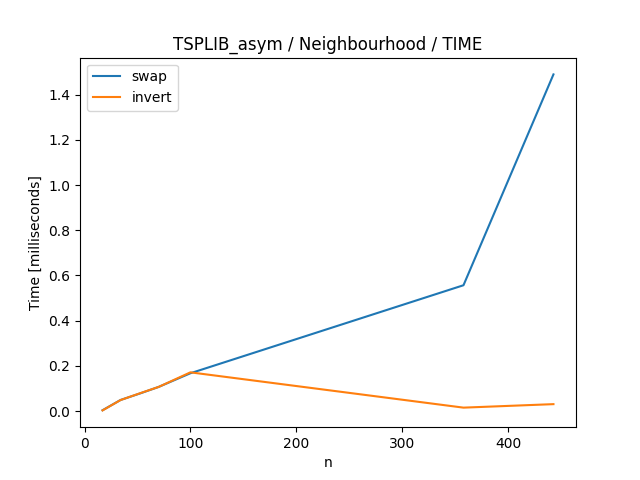
\includegraphics[width=\textwidth, 
                   height = 0.4\textheight, 
                   keepaspectratio]
                  {plots/neighbours_tsplib_asym_time} 
\end{center}

\subsubsection{Grafy euklidesowe}

\begin{center}
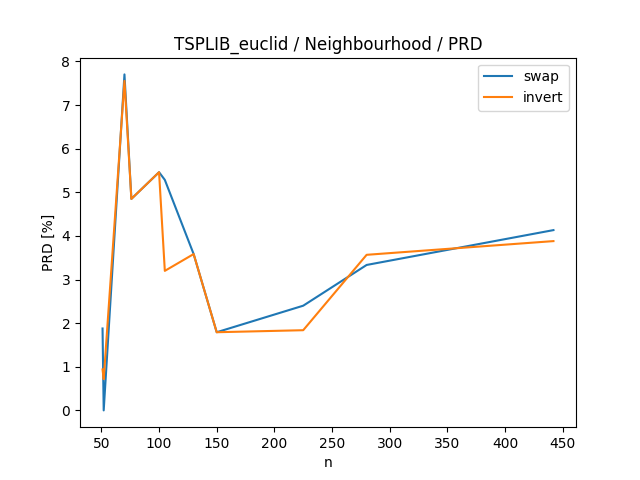
\includegraphics[width=\textwidth, 
                   height = 0.4\textheight, 
                   keepaspectratio]
                  {plots/neighbours_tsplib_euclid_prd} 
\end{center}

\begin{center}
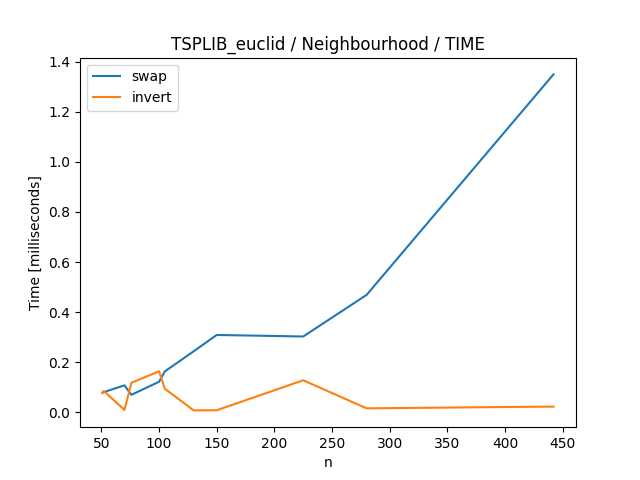
\includegraphics[width=\textwidth, 
                   height = 0.4\textheight, 
                   keepaspectratio]
                  {plots/neighbours_tsplib_euclid_time} 
\end{center}


\subsection{Dane generowane przez nas}


\subsubsection{Grafy symetryczne}

\begin{center}
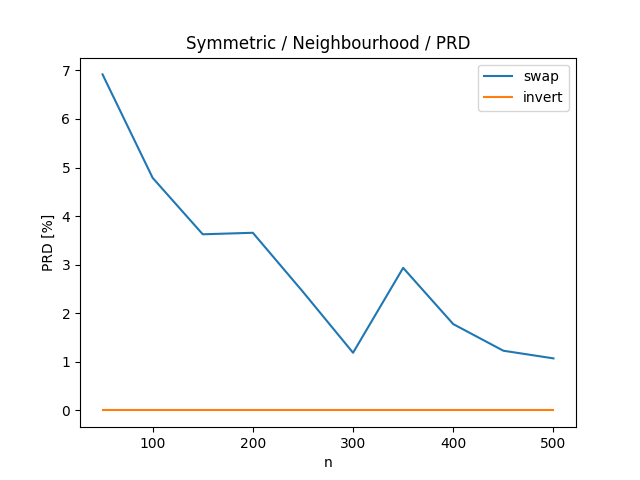
\includegraphics[width=\textwidth, 
                   height = 0.4\textheight, 
                   keepaspectratio]
                  {plots/neighbours_symmetric_prd} 
\end{center}

\begin{center}
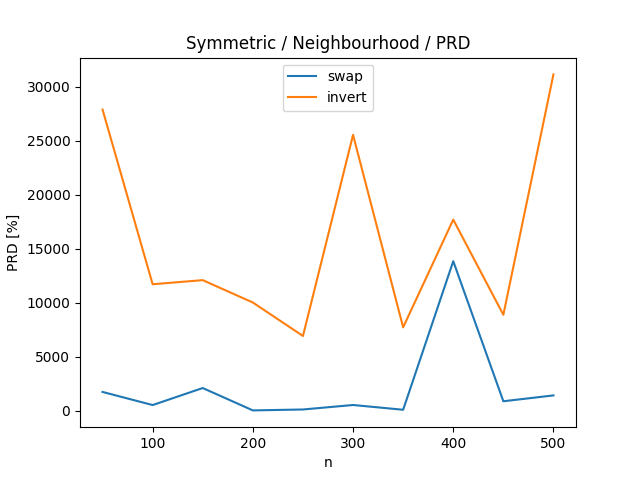
\includegraphics[width=\textwidth, 
                   height = 0.4\textheight, 
                   keepaspectratio]
                  {plots/neighbours_symmetric_time} 
\end{center}

\subsubsection{Grafy asymetryczne}

\begin{center}
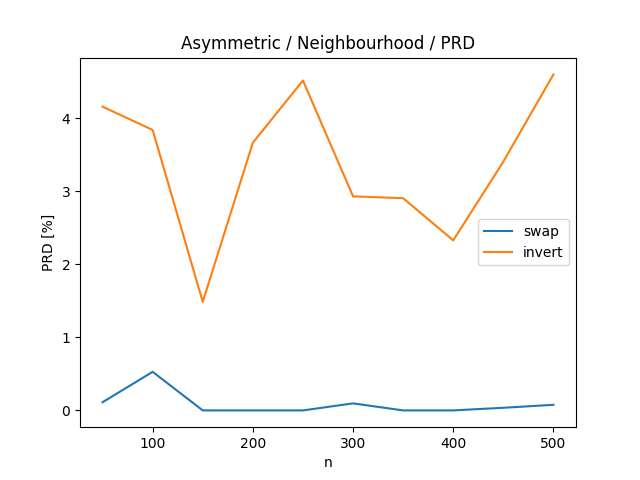
\includegraphics[width=\textwidth, 
                   height = 0.4\textheight, 
                   keepaspectratio]
                  {plots/neighbours_asymmetric_prd} 
\end{center}

\begin{center}
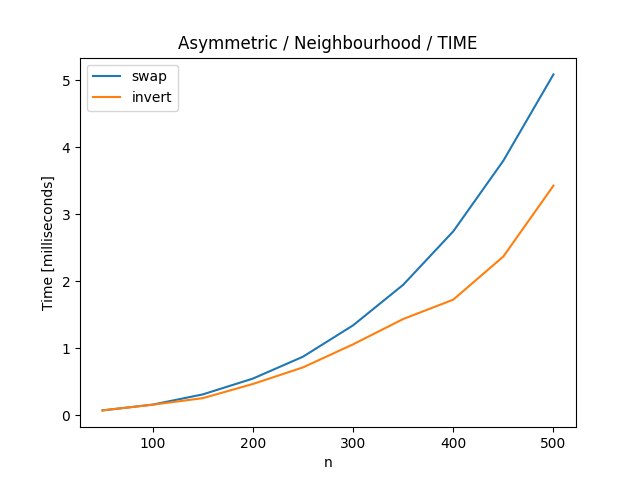
\includegraphics[width=\textwidth, 
                   height = 0.4\textheight, 
                   keepaspectratio]
                  {plots/neighbours_asymmetric_time} 
\end{center}

\subsubsection{Grafy euklidesowe}

\begin{center}
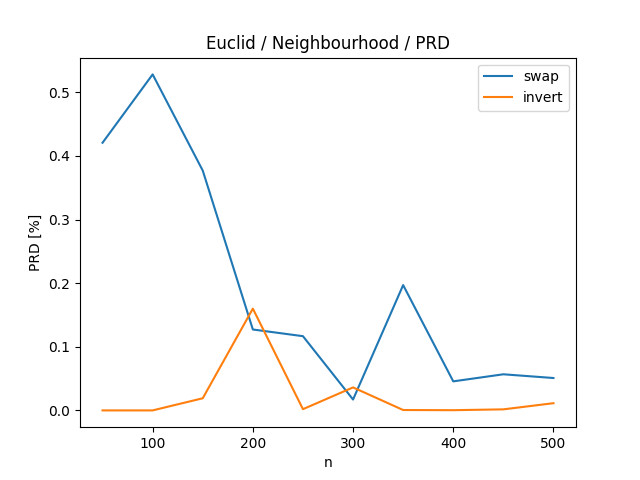
\includegraphics[width=\textwidth, 
                   height = 0.4\textheight, 
                   keepaspectratio]
                  {plots/neighbours_euclid_prd} 
\end{center}

\begin{center}
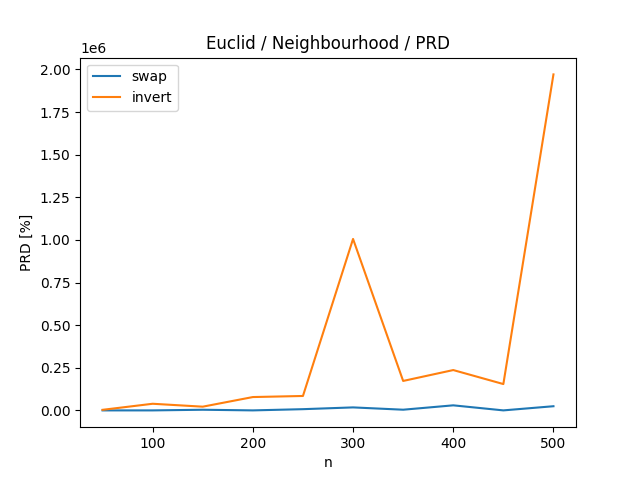
\includegraphics[width=\textwidth, 
                   height = 0.4\textheight, 
                   keepaspectratio]
                  {plots/neighbours_euclid_time} 
\end{center}

\subsection{Obserwacje}

Dla grafów asymetrycznych, lepszym wyborem jest sąsiedztwo swap - jest ono wyraźnie lepsze pod kątem jakości rozwiązania, natomiast wykonuje się dłużej.

Dla grafów symetrycznych rozwiązania uzyskane z użyciem otoczenia invert okazały się lepsze zarówno pod kątem jakości, jak i czasu.

W przypadku grafów euklidesowych, dla danych z TSPLIB oba sąsiedztwa dawały zbliżone wyniki, a dla danych generowanych przez nas lepsze było najczęściej sąsiedztwo invert (lecz dla większych $n$ nie była to wielka przewaga. Czasowo, tak jak w poprzednich grupach, zwycięzcą okazał się invert.

\subsection{Tabele}

\begin{center}
\begin{tabular}{|c|c|c|}
\hline
\multicolumn{3}{|c|}{\textbf{Asymmetric / Neighbourhood / PRD}}\\
\hline
\textbf{n} & Swap & Invert\\
\hline
50 & 0.11191047162270185 & 4.158695674522066\\
\hline
100 & 0.52807735217553 & 3.8398777948595333\\
\hline
150 & 0.0 & 1.4858723898734574\\
\hline
200 & 0.0 & 3.6649730337912074\\
\hline
250 & 0.0 & 4.5168141129407395\\
\hline
300 & 0.09599191647019198 & 2.930695727694611\\
\hline
350 & 0.0 & 2.9052223793423044\\
\hline
400 & 0.0 & 2.32776759746732\\
\hline
450 & 0.03581064508216826 & 3.4065936038225146\\
\hline
500 & 0.0766979513573519 & 4.6002407510123104\\
\hline
\end{tabular}
\end{center}


\begin{center}
\begin{tabular}{|c|c|c|}
\hline
\multicolumn{3}{|c|}{\textbf{Asymmetric / Neighbourhood / Time}}\\
\hline
\textbf{n} & Swap & Invert\\
\hline
50 & 0.07376404 & 0.07431734000000001\\
\hline
100 & 0.16007074999999998 & 0.1585202\\
\hline
150 & 0.31249241000000005 & 0.25652474\\
\hline
200 & 0.54841901 & 0.46782404\\
\hline
250 & 0.8751694499999999 & 0.7156449800000001\\
\hline
300 & 1.34324706 & 1.05975427\\
\hline
350 & 1.9484998399999998 & 1.4376728399999998\\
\hline
400 & 2.74655025 & 1.72702253\\
\hline
450 & 3.801825290000001 & 2.37098031\\
\hline
500 & 5.08990898 & 3.4289974899999995\\
\hline
\end{tabular}
\end{center}


\begin{center}
\begin{tabular}{|c|c|c|}
\hline
\multicolumn{3}{|c|}{\textbf{Euclid / Neighbourhood / PRD}}\\
\hline
\textbf{n} & Swap & Invert\\
\hline
50 & 0.4207549708890032 & 0.0\\
\hline
100 & 0.5282007435256711 & 0.0\\
\hline
150 & 0.3769823007501678 & 0.019084422822491107\\
\hline
200 & 0.1271843910979231 & 0.1599885829684126\\
\hline
250 & 0.11667189906458164 & 0.001928268414963363\\
\hline
300 & 0.017076672487704073 & 0.03614358129615766\\
\hline
350 & 0.19697835915506468 & 0.0005993048064245475\\
\hline
400 & 0.04564711832989831 & 0.0003221130616846514\\
\hline
450 & 0.056766273647667766 & 0.0016375098932889388\\
\hline
500 & 0.050901971434817714 & 0.011337910696104788\\
\hline
\end{tabular}
\end{center}


\begin{center}
\begin{tabular}{|c|c|c|}
\hline
\multicolumn{3}{|c|}{\textbf{Euclid / Neighbourhood / Time}}\\
\hline
\textbf{n} & Swap & Invert\\
\hline
50 & 0.4207549708890032 & 0.0\\
\hline
50 & 0.07344694 & 0.07000031999999999\\
\hline
100 & 0.16274169 & 0.12673666\\
\hline
150 & 0.3153742 & 0.16559282\\
\hline
200 & 0.5656857900000001 & 0.23007239999999998\\
\hline
250 & 0.89462399 & 0.39235521999999995\\
\hline
300 & 1.37161821 & 0.17630289\\
\hline
350 & 2.0154079099999995 & 0.64804025\\
\hline
400 & 2.8054042600000004 & 0.30653431\\
\hline
450 & 3.8271469 & 0.74014913\\
\hline
500 & 5.11919333 & 1.0551518899999999\\
\hline
\end{tabular}
\end{center}


\begin{center}
\begin{tabular}{|c|c|c|}
\hline
\multicolumn{3}{|c|}{\textbf{Symmetric / Neighbourhood / PRD}}\\
\hline
\textbf{n} & Swap & Invert\\
\hline
50 & 6.917692987893891 & 0.0\\
\hline
100 & 4.787518110638111 & 0.0\\
\hline
150 & 3.6259066537639213 & 0.0\\
\hline
200 & 3.65693454118884 & 0.0\\
\hline
250 & 2.4413015900221464 & 0.0\\
\hline
300 & 1.1869594271627262 & 0.0\\
\hline
350 & 2.9343241182614768 & 0.0\\
\hline
400 & 1.7767045918185538 & 0.0\\
\hline
450 & 1.2285915175711815 & 0.0\\
\hline
500 & 1.0711060843000912 & 0.0\\
\hline
\end{tabular}
\end{center}

\begin{center}
\begin{tabular}{|c|c|c|}
\hline
\multicolumn{3}{|c|}{\textbf{Symmetric / Neighbourhood / Time}}\\
\hline
\textbf{n} & Swap & Invert\\
\hline
50 & 0.07261012 & 0.06425642\\
\hline
100 & 0.16149818 & 0.08848346\\
\hline
150 & 0.30667559000000005 & 0.11450532\\
\hline
200 & 0.54723579 & 0.18917302\\
\hline
250 & 0.8675596299999999 & 0.22676869000000002\\
\hline
300 & 1.33364641 & 0.51011874\\
\hline
350 & 1.95661837 & 0.35503858\\
\hline
400 & 2.7663511699999996 & 1.01861845\\
\hline
450 & 3.79851777 & 1.75846868\\
\hline
500 & 5.06103543 & 0.95719657\\
\hline
\end{tabular}
\end{center}


\begin{center}
\begin{tabular}{|c|c|c|}
\hline
\multicolumn{3}{|c|}{\textbf{TSPLIB asym / Neighbourhood / PRD}}\\
\hline
\textbf{n} & Swap & Invert\\
\hline
17 & 0.0 & 0.0\\
\hline
34 & 5.365474339035769 & 16.018662519440124\\
\hline
53 & 16.437364228819696 & 17.465604634322954\\
\hline
70 & 4.881958989475862 & 5.662865565122955\\
\hline
100 & 11.783052718741374 & 13.773116202042507\\
\hline
358 & 14.531384350816854 & 48.92519346517627\\
\hline
443 & 4.338235294117647 & 41.43382352941177\\
\hline
\end{tabular}
\end{center}


\begin{center}
\begin{tabular}{|c|c|c|}
\hline
\multicolumn{3}{|c|}{\textbf{TSPLIB asym / Neighbourhood / Time}}\\
\hline
\textbf{n} & Swap & Invert\\
\hline
17 & 0.0034579 & 0.0027282\\
\hline
34 & 0.0488397 & 0.0485128\\
\hline
53 & 0.0787211 & 0.0796033\\
\hline
70 & 0.1066343 & 0.1066752\\
\hline
100 & 0.1671848 & 0.1711747\\
\hline
358 & 0.556717 & 0.0149537\\
\hline
443 & 1.4899777 & 0.0304211\\
\hline
\end{tabular}
\end{center}


\begin{center}
\begin{tabular}{|c|c|c|}
\hline
\multicolumn{3}{|c|}{\textbf{TSPLIB euclid / Neighbourhood / PRD}}\\
\hline
\textbf{n} & Swap & Invert\\
\hline
51 & 1.8779342723004695 & 0.9389671361502347\\
\hline
52 & 0.0 & 0.7159904534606205\\
\hline
70 & 7.703703703703704 & 7.555555555555555\\
\hline
76 & 4.849342172172451 & 4.849342172172451\\
\hline
100 & 5.461441213653603 & 5.461441213653603\\
\hline
105 & 5.285485777870505 & 3.1991098129216216\\
\hline
130 & 3.5842880523731586 & 3.5842880523731586\\
\hline
150 & 1.7922794117647058 & 1.7922794117647058\\
\hline
225 & 2.400408580183861 & 1.8386108273748722\\
\hline
280 & 3.3346258239627766 & 3.5672741372625048\\
\hline
442 & 4.133679940131553 & 3.881602268699043\\
\hline
\end{tabular}
\end{center}


\begin{center}
\begin{tabular}{|c|c|c|}
\hline
\multicolumn{3}{|c|}{\textbf{TSPLIB euclid / Neighbourhood / Time}}\\
\hline
\textbf{n} & Swap & Invert\\
\hline
51 & 0.0792794 & 0.0792618\\
\hline
52 & 0.0793002 & 0.0792362\\
\hline
70 & 0.1098126 & 0.0094275\\
\hline
76 & 0.113911 & 0.1344349\\
\hline
100 & 0.1608226 & 0.155615\\
\hline
105 & 0.1828318 & 0.1793799\\
\hline
130 & 0.2498604 & 0.0066768\\
\hline
150 & 0.3236019 & 0.0076471\\
\hline
225 & 0.6941704 & 0.1050844\\
\hline
280 & 1.1307793 & 0.0139994\\
\hline
442 & 3.5502116 & 0.0242614\\
\hline
\end{tabular}
\end{center}



\section{Porównanie wersji wielowątkowej i wersji jednowątkowej}

\subsection{Dane z TSPLIB}

\subsubsection{Grafy asymetryczne}

\begin{center}
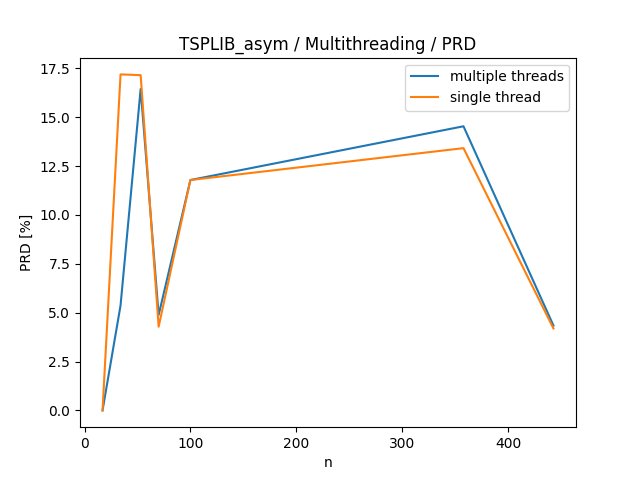
\includegraphics[width=\textwidth, 
                   height = 0.4\textheight, 
                   keepaspectratio]
                  {plots/multithreading_tsplib_asym_prd} 
\end{center}

\begin{center}
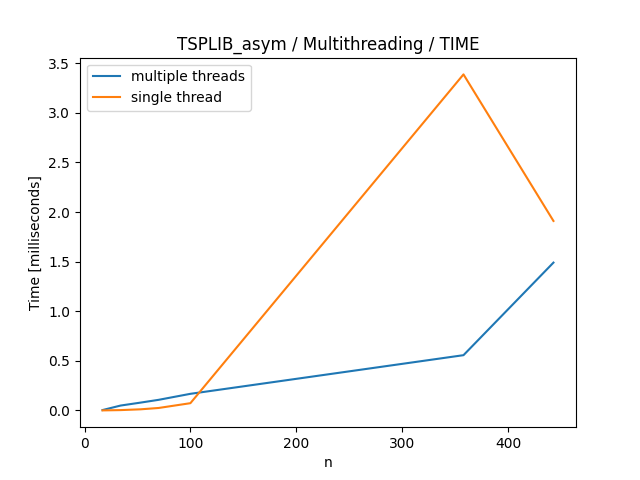
\includegraphics[width=\textwidth, 
                   height = 0.4\textheight, 
                   keepaspectratio]
                  {plots/multithreading_tsplib_asym_time} 
\end{center}

\subsubsection{Grafy euklidesowe}

\begin{center}
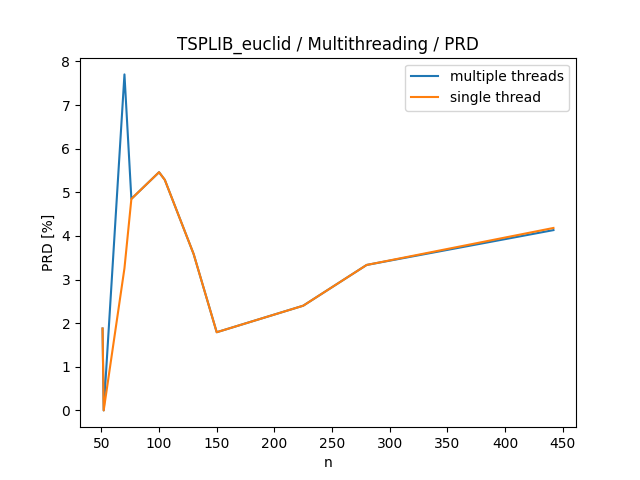
\includegraphics[width=\textwidth, 
                   height = 0.4\textheight, 
                   keepaspectratio]
                  {plots/multithreading_tsplib_euclid_prd} 
\end{center}

\begin{center}
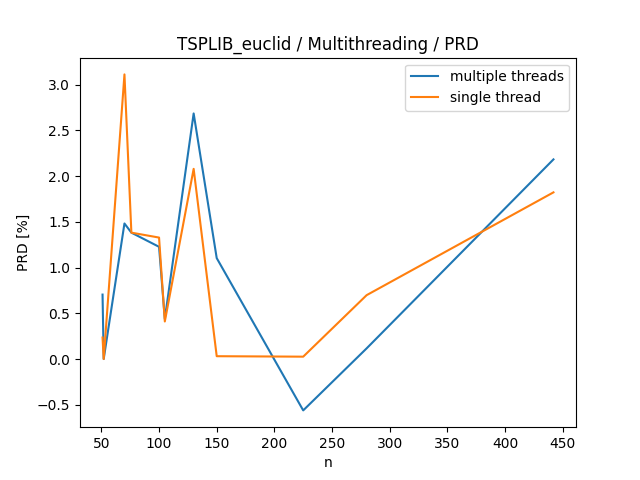
\includegraphics[width=\textwidth, 
                   height = 0.4\textheight, 
                   keepaspectratio]
                  {plots/multithreading_tsplib_euclid_time} 
\end{center}


\subsection{Dane generowane przez nas}


\subsubsection{Grafy symetryczne}

\begin{center}
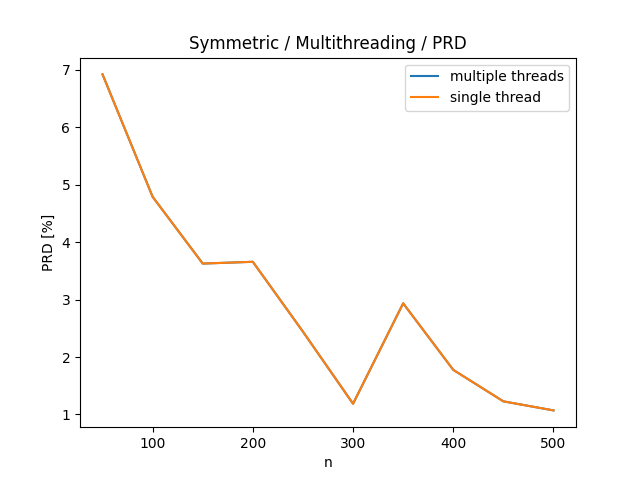
\includegraphics[width=\textwidth, 
                   height = 0.4\textheight, 
                   keepaspectratio]
                  {plots/multithreading_symmetric_prd} 
\end{center}

\begin{center}
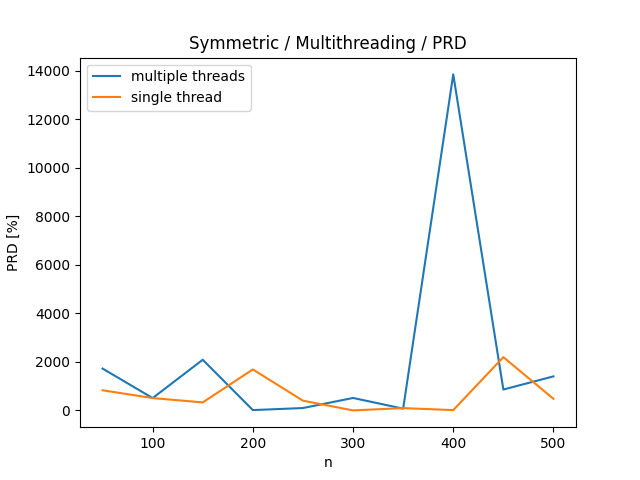
\includegraphics[width=\textwidth, 
                   height = 0.4\textheight, 
                   keepaspectratio]
                  {plots/multithreading_symmetric_time} 
\end{center}

\subsubsection{Grafy asymetryczne}

\begin{center}
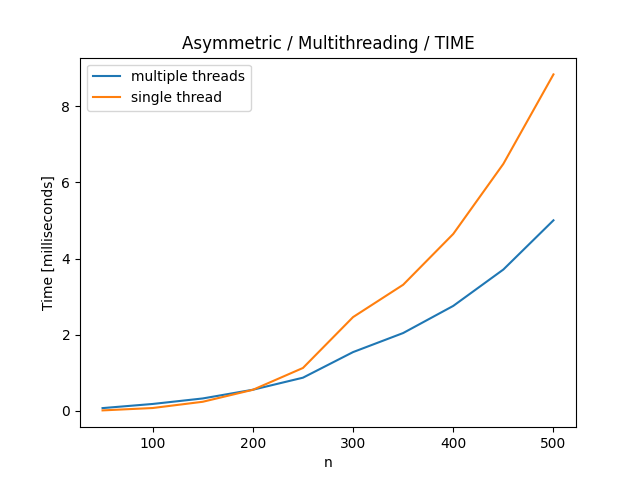
\includegraphics[width=\textwidth, 
                   height = 0.4\textheight, 
                   keepaspectratio]
                  {plots/multithreading_asymmetric_prd} 
\end{center}

\begin{center}
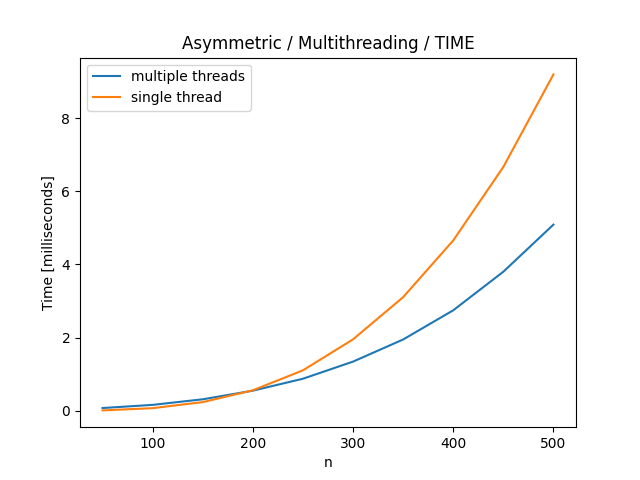
\includegraphics[width=\textwidth, 
                   height = 0.4\textheight, 
                   keepaspectratio]
                  {plots/multithreading_asymmetric_time} 
\end{center}

\subsubsection{Grafy euklidesowe}

\begin{center}
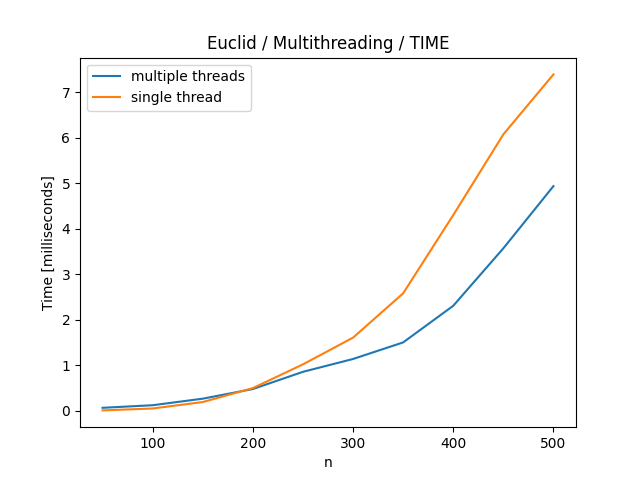
\includegraphics[width=\textwidth, 
                   height = 0.4\textheight, 
                   keepaspectratio]
                  {plots/multithreading_euclid_prd} 
\end{center}

\begin{center}
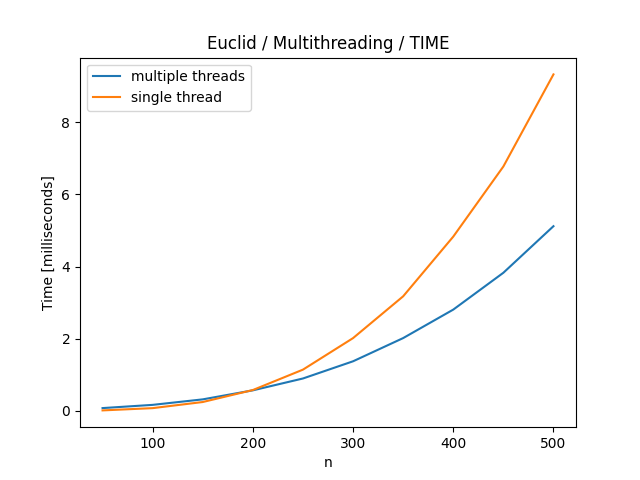
\includegraphics[width=\textwidth, 
                   height = 0.4\textheight, 
                   keepaspectratio]
                  {plots/multithreading_euclid_time} 
\end{center}

\subsection{Obserwacje}

PRD dla wersji jedno- oraz wielowątkowej było bardzo zbliżone, albo dokładnie takie samo. Czasowo dla najmniejszych grafów minimalnie wygrywała wersja bez współbieżności, natomiast dla większych macierzy zdecydowanie lepsza była wersja z wątkami.

\subsection{Tabele}

\begin{center}
\begin{tabular}{|c|c|c|}
\hline
\multicolumn{3}{|c|}{\textbf{Asymmetric / Multithreading / PRD}}\\
\hline
\textbf{n} & Multiple threads & Single thread\\
\hline
50 & 0.11191047162270185 & 0.11191047162270185\\
\hline
100 & 0.52807735217553 & 0.52807735217553\\
\hline
150 & 0.0 & 0.0\\
\hline
200 & 0.0 & 0.0\\
\hline
250 & 0.0 & 0.0\\
\hline
300 & 0.09599191647019198 & 0.09599191647019198\\
\hline
350 & 0.0 & 0.0\\
\hline
400 & 0.0 & 0.0\\
\hline
450 & 0.03581064508216826 & 0.03581064508216826\\
\hline
500 & 0.0766979513573519 & 0.0766979513573519\\
\hline
\end{tabular}
\end{center}


\begin{center}
\begin{tabular}{|c|c|c|}
\hline
\multicolumn{3}{|c|}{\textbf{Asymmetric / Multithreading / Time}}\\
\hline
\textbf{n} & Multiple threads & Single thread\\
\hline
50 & 0.07376404 & 0.00903833\\
\hline
100 & 0.16007074999999998 & 0.07002836999999999\\
\hline
150 & 0.31249241000000005 & 0.23549518999999997\\
\hline
200 & 0.54841901 & 0.5584251\\
\hline
250 & 0.8751694499999999 & 1.10466398\\
\hline
300 & 1.34324706 & 1.951844\\
\hline
350 & 1.9484998399999998 & 3.1064202999999995\\
\hline
400 & 2.74655025 & 4.65695869\\
\hline
450 & 3.801825290000001 & 6.6676786\\
\hline
500 & 5.08990898 & 9.196990920000001\\
\hline
\end{tabular}
\end{center}


\begin{center}
\begin{tabular}{|c|c|c|}
\hline
\multicolumn{3}{|c|}{\textbf{Euclid / Multithreading / PRD}}\\
\hline
\textbf{n} & Multiple threads & Single thread\\
\hline
50 & 0.4207549708890032 & 0.4207549708890032\\
\hline
100 & 0.5282007435256711 & 0.5648531564761904\\
\hline
150 & 0.3769823007501678 & 0.3769823007501678\\
\hline
200 & 0.1271843910979231 & 0.1271843910979231\\
\hline
250 & 0.11667189906458164 & 0.11667189906458164\\
\hline
300 & 0.017076672487704073 & 0.017076672487704073\\
\hline
350 & 0.19697835915506468 & 0.19697835915506468\\
\hline
400 & 0.04564711832989831 & 0.04564711832989831\\
\hline
450 & 0.056766273647667766 & 0.056766273647667766\\
\hline
500 & 0.050901971434817714 & 0.05042549734309646\\
\hline
\end{tabular}
\end{center}


\begin{center}
\begin{tabular}{|c|c|c|}
\hline
\multicolumn{3}{|c|}{\textbf{Euclid / Multithreading / Time}}\\
\hline
\textbf{n} & Multiple threads & Single thread\\
\hline
50 & 0.07344694 & 0.009324530000000001\\
\hline
100 & 0.16274169 & 0.07212905\\
\hline
150 & 0.3153742 & 0.24179654\\
\hline
200 & 0.5656857900000001 & 0.57428542\\
\hline
250 & 0.89462399 & 1.14006875\\
\hline
300 & 1.37161821 & 2.0147588300000003\\
\hline
350 & 2.0154079099999995 & 3.17420528\\
\hline
400 & 2.8054042600000004 & 4.82983258\\
\hline
450 & 3.8271469 & 6.774824010000001\\
\hline
500 & 5.11919333 & 9.329994919999999\\
\hline
\end{tabular}
\end{center}


\begin{center}
\begin{tabular}{|c|c|c|}
\hline
\multicolumn{3}{|c|}{\textbf{Symmetric / Multithreading / PRD}}\\
\hline
\textbf{n} & Multiple threads & Single thread\\
\hline
50 & 6.917692987893891 & 6.917692987893891\\
\hline
100 & 4.787518110638111 & 4.787518110638111\\
\hline
150 & 3.6259066537639213 & 3.6259066537639213\\
\hline
200 & 3.65693454118884 & 3.65693454118884\\
\hline
250 & 2.4413015900221464 & 2.4413015900221464\\
\hline
300 & 1.1869594271627262 & 1.1869594271627262\\
\hline
350 & 2.9343241182614768 & 2.9343241182614768\\
\hline
400 & 1.7767045918185538 & 1.7767045918185538\\
\hline
450 & 1.2285915175711815 & 1.2285915175711815\\
\hline
500 & 1.0711060843000912 & 1.0711060843000912\\
\hline
\end{tabular}
\end{center}


\begin{center}
\begin{tabular}{|c|c|c|}
\hline
\multicolumn{3}{|c|}{\textbf{Symmetric / Multithreading / Time}}\\
\hline
\textbf{n} & Multiple threads & Single thread\\
\hline
50 & 0.07261012 & 0.00909796\\
\hline
100 & 0.16149818 & 0.07070326000000002\\
\hline
150 & 0.30667559000000005 & 0.23711314\\
\hline
200 & 0.54723579 & 0.55973583\\
\hline
250 & 0.8675596299999999 & 1.10501948\\
\hline
300 & 1.33364641 & 1.93088376\\
\hline
350 & 1.95661837 & 3.10280147\\
\hline
400 & 2.7663511699999996 & 4.66704174\\
\hline
450 & 3.79851777 & 6.665332530000001\\
\hline
500 & 5.06103543 & 9.190356060000001\\
\hline
\end{tabular}
\end{center}


\begin{center}
\begin{tabular}{|c|c|c|}
\hline
\multicolumn{3}{|c|}{\textbf{TSPLIB asym / Multithreading / PRD}}\\
\hline
\textbf{n} & Multiple threads & Single thread\\
\hline
17 & 0.0 & 0.0\\
\hline
34 & 5.365474339035769 & 17.1850699844479\\
\hline
53 & 16.437364228819696 & 17.14699493120927\\
\hline
70 & 4.881958989475862 & 4.282057249243659\\
\hline
100 & 11.783052718741374 & 11.783052718741374\\
\hline
358 & 14.531384350816854 & 13.413585554600171\\
\hline
443 & 4.338235294117647 & 4.191176470588235\\
\hline
\end{tabular}
\end{center}


\begin{center}
\begin{tabular}{|c|c|c|}
\hline
\multicolumn{3}{|c|}{\textbf{TSPLIB asym / Multithreading / Time}}\\
\hline
\textbf{n} & Multiple threads & Single thread\\
\hline
17 & 0.0034579 & 4.27e-05\\
\hline
34 & 0.0488397 & 0.0030225\\
\hline
53 & 0.0787211 & 0.011016\\
\hline
70 & 0.1066343 & 0.0245621\\
\hline
100 & 0.1671848 & 0.0727892\\
\hline
358 & 0.556717 & 3.387291\\
\hline
443 & 1.4899777 & 1.9098416\\
\hline
\end{tabular}
\end{center}


\begin{center}
\begin{tabular}{|c|c|c|}
\hline
\multicolumn{3}{|c|}{\textbf{TSPLIB euclid / Multithreading / PRD}}\\
\hline
\textbf{n} & Multiple threads & Single thread\\
\hline
51 & 1.8779342723004695 & 1.8779342723004695\\
\hline
52 & 0.0 & 0.0\\
\hline
70 & 7.703703703703704 & 3.259259259259259\\
\hline
76 & 4.849342172172451 & 4.849342172172451\\
\hline
100 & 5.461441213653603 & 5.461441213653603\\
\hline
105 & 5.285485777870505 & 5.285485777870505\\
\hline
130 & 3.5842880523731586 & 3.5842880523731586\\
\hline
150 & 1.7922794117647058 & 1.7922794117647058\\
\hline
225 & 2.400408580183861 & 2.400408580183861\\
\hline
280 & 3.3346258239627766 & 3.3346258239627766\\
\hline
442 & 4.133679940131553 & 4.182913860333215\\
\hline
\end{tabular}
\end{center}


\begin{center}
\begin{tabular}{|c|c|c|}
\hline
\multicolumn{3}{|c|}{\textbf{TSPLIB euclid / Multithreading / Time}}\\
\hline
\textbf{n} & Multiple threads & Single thread\\
\hline
51 & 0.0792794 & 0.0099841\\
\hline
52 & 0.0793002 & 0.0112551\\
\hline
70 & 0.1098126 & 0.0257936\\
\hline
76 & 0.113911 & 0.0326535\\
\hline
100 & 0.1608226 & 0.072437\\
\hline
105 & 0.1828318 & 0.0835306\\
\hline
130 & 0.2498604 & 0.1702319\\
\hline
150 & 0.3236019 & 0.2482995\\
\hline
225 & 0.6941704 & 0.8124654\\
\hline
280 & 1.1307793 & 1.6300746\\
\hline
442 & 3.5502116 & 6.2351401\\
\hline
\end{tabular}
\end{center}



\section{Wnioski}
\begin{itemize}
\item Algorytm przeszukiwania z zabronieniami zawsze podaje co najmniej tak samo dobry wynik jak $2-OPT$, ponieważ przyjmuje jego wynik za przybliżenie początkowe. Oba algorytmy działają najlepiej dla grafów euklidesowych, a największe polepszenie wyniku jest dla grafów asymetrycznych. Jest tak dlatego, że w grafach asymetrycznych łatwo znaleźć lokalne minimum, które jest dalekie od globalnego, natomiast grafy euklidesowe mają lokalne minima bliskie globalnemu.
\item Dla różnych długości listy zabronień ($13, \sqrt{n}, n$) znalezione najkrótsze ścieżki we wszystkich rodzinach grafów są identyczne lub bardzo bliskie sobie. Natomiast czas działania algorytmu rośnie dla większych długości, bo przeglądanie listy zabronień jest dłuższe. Dla grafów do $n=500$ wartość $13$ zapewnia najlepszy czas działania i bardzo dobre wyniki.
\item W grafach euklidesowych i symetrycznych sąsiedztwo $invert$ znajduje lepsze rozwiązania w krótszym czasie (warunek wyjścia to nieznalezienie lepszego rozwiązania przez $n$ ruchów). Natomiast w grafach asymetrycznych sąsiedztwo $swap$ daje lepsze wyniki - w grafach asymetrycznych $invert$ może często przedłużyć znalezioną ścieżkę.
\item Wersja jednowątkowa i wielowątkowa dają niemal identyczne wyniki - różnice wynikają z tego, że wątki mogą kończyć w różnym czasie swoje działania i dlatego wynik jest inny niż w jednym wątku. Dla małych grafów komunikacja między wątkami jest droga i pogarsza czas działania, natomiast dla większych grafów ($n\geq 200$) czas działania algorytmu współbieżnego jest prawie dwukrotnie mniejszy, ponieważ koszta przesyłania danych między wątkami są nadrabiane przez równoległe obliczenia.  
\end{itemize}

\end{document}